\documentclass[conference]{IEEEtran}
\usepackage{ctex}
% CJK 主字体：ctex 默认字集 FandolSong 缺字形（PDF 会出现空白/方框），
% 必须用系统华文宋体 STSong（普通 TrueType，xdvipdfmx 可正常子集嵌入）。
% ⚠️ 不要用 Noto Serif SC：本机那版是可变字体 VF，会被 xdvipdfmx 以 Invalid TTC index 拒收。
\setCJKmainfont{STSong}
% IEEEtran 不带 natbib，\citep/\citet 会报 Undefined control sequence；
% 且必须带 [numbers]：只写 \usepackage{natbib} 会报
% Bibliography not compatible with author-year citations。
\usepackage[numbers]{natbib}
\usepackage{amsmath}
\usepackage{amssymb}
\usepackage{graphicx}
\usepackage{makecell}
\usepackage{booktabs}
\usepackage{tabulary}

% math_commands.tex —— 全文数学符号与缩略语统一定义（各篇可按需增删，勿改已有通用宏）
\newcommand{\kg}{知识图谱}
\newcommand{\corpus}{语料}
\newcommand{\salience}{叙事热度}
\newcommand{\centre}{中心性}
\newcommand{\Deg}{d}
\newcommand{\Chap}{h}
\newcommand{\Rho}{\rho}
\newcommand{\NP}{\emph{N}}
\newcommand{\bk}[1]{\textbf{#1}}
\newcommand{\cited}[1]{[\cite{#1}]}
\newcommand{\pct}[1]{#1\%}

% latex_includes.tex —— 只声明图片搜索路径与统一宽度宏
% ⚠️ 禁止在本文件里写 \begin{comment}...\end{comment} 包裹的示例 figure：
%    comment 环境需要 \usepackage{comment}，否则编译直接报
%    "LaTeX Error: Environment comment undefined"（试点篇踩过）。
% 所有 figure 环境一律写在 sections/5_results.tex 内，图题只进 \caption，图内不写标题。
\graphicspath{{figures/}}
\newcommand{\figpath}[1]{figures/#1}


% ⚠️ IEEEtran conference 类不定义 \bibname（那是 book/article 类的宏），
%    加 \renewcommand{\bibname}{...} 会直接编译失败。栏头沿用 venue 原有的英文 References。

\title{崩塌的涌现：复杂网络中的明朝兴衰——一部通俗明史叙事的度数、连通与危机迁移\\[2pt]
\large Emergent Collapse: Degree, Connectivity and Crisis Shift in a Ming Knowledge Graph}

\author{Anonymous}
\date{}

\begin{document}
\maketitle

\noindent\textbf{摘要（中文）}：本文把「明朝的兴衰是一个涌现过程」这一说法压到可计算的位置，
不是复述它，而是检验它在什么数据上成立、在什么数据上必须收手。
语料是同一部通俗明史叙事的结构化知识图谱：1231 位人物、2324 条关系、1106 件事件、563 处地点。
度数分布高度集中：基尼系数 0.8199，537 人（43.6\%）无任何关系，
度数排序前一百的人（占全体的 8.8\%）握有全部度数和的 65.1\%；
但把度数序列套进 Hill 估计器时会发现 α̂ 随 xmin 从 1.806 一路走到 2.777，
漂移 0.971，而尾样本只有 142 条——据此本篇明确不主张幂律，
并把「复杂」落成可复核的另外两个量：基尼系数与最大连通块占比。
连通性一侧给出 741 个带边的顶点、18 个连通块，最大块 703 点，
占带边顶点的 94.9\%，却只占全部人物的 57.1\%——图是连通的，人物不是。
时间一侧，1006 件事件落在 1328—1645 的 218 个年份上，
年均 4.615 件、变异系数 1.16、按年基尼 0.5069；
按 1368—1499 / 1500—1599 / 1600—1662 三期切分，
事件类别分布 χ²=129.05（df=20，p 小于 $10^{-6}$），Cramér's V=0.259：
军事战争由 28.9\% 降到 21.8\% 再抬到 40.9\%，
政治斗争由 33.9\% 升到 40.8\% 再落到 21.5\%——危机不是同一类危机的持续，是类别的换位。
全部数字可复算。

\noindent\textbf{关键词}：复杂网络；度数集中；连通块；幂律边界；危机类别迁移；数字人文

\vspace{6pt}
\begin{abstract}
We ask whether the claim that a dynasty's rise and fall is an emergent process can be
pinned to quantities that recompute, rather than repeated as a metaphor. The corpus is a
structured knowledge graph over a widely read popular Ming narrative: 1231 persons, 2324
relations, 1106 dated events, 563 places. Degree is sharply concentrated: the Gini
coefficient is 0.8199, 537 persons (43.6\%) have no relation at all, and the 108 persons
at the top of the degree order hold 65.1 percent of the total degree mass. Yet when the
degree sequence is passed to a Hill estimator, the estimated exponent drifts from 1.806 to
2.777 as the cutoff xmin rises, a spread of 0.971 on a tail of 142 observations; we
therefore decline to claim a power law and instead report two robust quantities, the Gini
coefficient and the share of the largest connected component. On connectivity the graph is
one piece: 741 vertices carry edges, there are 18 components, and the largest holds 703
vertices, 94.9 percent of edge-bearing vertices but only 57.1 percent of all persons. In
time, 1006 events fall on 218 distinct years (1328--1645) with a mean of 4.615 per year,
a coefficient of variation of 1.16 and a year-wise Gini of 0.5069. Splitting into
1368--1499, 1500--1599 and 1600--1662, the event-category distribution moves with
chi-square 129.05 on 20 degrees of freedom and Cramer's V of 0.259: military conflict goes
28.9, 21.8, 40.9 percent while political contest goes 33.9, 40.8, 21.5 percent. The crisis
is not one crisis sustained; it is a change of category. Every figure recomputes.
\end{abstract}

\begin{IEEEkeywords}
complex networks, degree concentration, connected components, power-law boundaries, crisis category shift, digital humanities
\end{IEEEkeywords}

\section{引言}

「明朝是一个复杂系统，它的灭亡是涌现出来的」——这句话今天很常见，也很少被算过。
涌现（emergence）在复杂网络研究里不是一句形容：它要求一个系统的宏观形状
既不等于任何单个成员的性质，又是从成员之间的连接规则里长出来的。
把这句话搬到一部叙事抽取出的知识图谱上，它就变成一组可算的量：
度数分布有多集中、分布是不是幂律、图是不是一整块、连接的形状随时间怎么移。
本篇要做的不是复述"兴衰=涌现"，而是先把它拆成可复核的四个量，
再报告其中哪些算得出来、哪些在现有样本量下必须收手。

具体问法是四个问题。\textbf{第一，这部叙事写的人有多集中：}
1231 位人物里，有多少人一条关系也没有，度数的分布形状是平台还是长尾。
\textbf{第二，这个形状能不能叫无标度：}
按 Clauset 等人对幂律拟合的要求，尾指数应当在大样本上是稳的；
若它随截断点的抬升系统性漂移，那么"幂律"这一标签就不该贴上去。
\textbf{第三，图是不是连通的：}
一个 dynastic 叙事的网络通常被渲染成一张密网，但密网是可以由少数枢纽撑起来的假象。
\textbf{第四，这个形状有没有随时间换位：}
若"崩塌"真的在书写中被感知为一个过程，事件类别的比重应当在三期之间迁移，
而不只是总量变化。

语料是通俗明史叙事《明朝那些事儿》全七部，以及从同一语料抽取、可独立重建的
结构化知识图谱：人物 1231、事件 1106、关系 2324 条、地点 563 处。
其中 1006 件事件带可解析年份，落在 1328—1645 之间的 218 个年份上。
本篇量的不是明朝是否真亡于某个原因，而是这部被读过最多的叙事，
在结构上长成了什么样的一张图。

结果指向一个清楚的形状。度数侧高度集中但不必称幂律：
基尼系数 0.8199，537 人（43.6\%）一条关系也没有，
度数排序前一百的 108 人（占全部人物的 8.8\%）握有全部度数和的 65.1\%，
尾指数估计值却随 xmin 从 1.806 一路漂到 2.777（漂移 0.971，尾样本仅 142 条）。
连通侧是一整块：741 个顶点带边、18 个连通块、最大块 703 点，
占带边顶点的 94.9\%，只占全部人物的 57.1\%。
时间侧不是均匀增长：年均 4.615 件、变异系数 1.16、按年基尼 0.5069，
而 1368—1499 / 1500—1599 / 1600—1662 三期之间的事件类别分布
χ²=129.05（df=20，p 小于 $10^{-6}$），Cramér's V=0.259。

贡献有三点。
\begin{itemize}
\item 把"兴衰是涌现"拆成四个可复算的量：集中（基尼）、分布形状（尾指数稳定性）、
连通（最大连通块占比）、时间迁移（类别占比的三期位移），每一个都给出点数的口径。
\item 明确一条负结果——本篇不主张幂律，并把"在多大的尾样本上必须放弃幂律主张"
写成一条可复核的判据（第 6 节），而不是留作脚注。
\item 报一个可用卡方复核的时期迁移：军事战争占比 28.9 / 21.8 / 40.9，
政治斗争占比 33.9 / 40.8 / 21.5，两者在第三期方向相反。
\end{itemize}

边界先说死：本篇不主张这套网络形状对应明代社会的真实结构，
也不主张"崩塌"二字落在哪一年。它量的是一部叙事在抽取之后长成的形状。

第 2 节回顾相关文献，第 3 节交代语料与口径，第 4 节写方法，
第 5 节报告结果，第 6 节讨论效度边界与幂律的样本量上限，第 7 节收束。

\section{相关工作}

本文压在四支文献的交汇处；每支既给口径，也给出本篇要绕开的那一步。

\textbf{复杂网络的骨架一支。}
随机图给了"平均度数为常"的基线，而 \citet{barabasi1999} 指出真实网络的度数分布
是无标度的——少数枢纽扛起绝大部分连接。本篇正落在这一支里，
但只取它的一半结论：枢纽确实存在（最大度数 113，单人占全部度数和的 2.5\%），
本篇不去论证"因此是无标度"，而去检验这个标签在数据上是否站得住（第 5.2 节）。
\citet{watts1998} 的小世界与 \citet{albert2000} 的攻击容忍度进一步说明：
一张看起来很密的网，可以只靠极少数节点连着，抽掉它们就散。
本篇第 5.3 节报的"18 个连通块、最大块占带边顶点的 94.9\%"，就是这条警告的直接读数。

\textbf{幂律拟合的边界一支，本篇主要借这一支。}
\citet{clauset2009} 给出了幂律拟合的完整判据：尾指数必须在大样本、多切点上稳定，
$x_{\min}$ 的选取要能自证，拟合优度要用连续检验而非分箱比较。
本篇第 5.2 节完全按这套口径去做，得到的是一条负结果：
尾指数随 xmin 漂移 0.971、尾样本只有 142 条，故不贴幂律标签。
把"复杂网络的常见形状"直接写进历史叙事研究的做法，
在没有走这一道检验之前，本篇一律不采用。
\textbf{网络方法进入历史学的一支。}
\citet{lemercier2015} 论证历史学者如何用网络方法，并点明首要陷阱：
从历史文本抽出的关系是叙述者建构的关系，不是被研究时代里发生过的关系。
本篇因此不复现任何"明代社会真实结构"的论断，只报这部叙事自己长成的形状。
\textbf{历史动力学一支，本篇借它作对照假设而不作证据。}
\citet{turchin2003} 主张历史宏观过程可用人口—财政的周期模型解释，
\citet{diamond2005} 则从多个社会比较"选择失败还是存活"。
两支都给了一个可对照的直觉：崩塌是结构性位移，不是单次事件。
本篇能验的只有其中一个可数项——结构位移在时间上是否真的发生了（第 5.5 节的类别迁移），
而且验的是文本抽取出来的事件类别，不是人口或财政数据。
方法层面本量级（1231 个顶点、2324 条边）的网络综述口径取自
\citet{newman2005} 与 \citet{wasserman1994}；本篇的基尼、连通块、
秩相关一律按这两支的定义算。

\textbf{本文的位置。}
四支里没有一支把"王朝兴衰"这个对象上的四个量（集中、幂律边界、连通、时间迁移）
同时点数出来：网络那两支给了形状与判据，历史学那两支给了对照假设与陷阱，
中间缺一层——用一个具体语料把这四个量一次算齐，并显式负报其中不成立者。
本篇用同一份图谱一次补齐，且把"不主张幂律"与"样本量上限"写进正文而非脚注。

\section{语料与口径}

\subsection{语料与抽取产物}

本文语料是通俗明史叙事《明朝那些事儿》全七部（2006 年起连载出版），
以及在其之上抽取的结构化知识图谱。图谱不是原书本身，而是原书的一次投影；
本篇的四个量全部建立在这一投影之上，第 6 节会反复回到这一点。

规模如表 \ref{tab:corpus} 所示。人物 1231、事件 1106、关系 2324、地点 563。
原书正文不外发，本章不做全文检索；事件类别的抽取由前序工序完成，
本篇只使用其分类结果，不重跑抽取，也不改写任何一条类别标签。

\begin{table}[!t]
\centering
\caption{语料与结构化抽取产物规模}
\label{tab:corpus}
\small
\begin{tabular}{lr}
\toprule
项目 & 数量 \\
\midrule
人物 & 1231 \\
事件 & 1106 \\
关系边 & 2324 \\
地点 & 563 \\
\bottomrule
\end{tabular}
\end{table}

\subsection{三条数据纪律}

本篇沿用项目统一的三条纪律，它们直接决定第 5 节的点数正确性。

\begin{itemize}
\item \textbf{裸名，无 id。} 关系记录的 from / to 存的是裸人物名（如「朱棣」），
人物表里没有 id 字段。凡按名字查表的地方一律用裸名，禁止按 id 拼串；
否则 2324 条边里会有成批的尸体边（端点落在人物表外）。
本篇剔除端点缺失或两端同名的记录后，带边顶点为 741 个（第 5.3 节）。
\item \textbf{坐标不按假值判空。} 地理维度在本篇不使用，因此这条不参与计算，
但凡涉及经纬度的地方必须写 `is None' 判空，不能写 `if not lat'——
0 是合法经纬度，写成假值会把坐标原点上的地点整批丢掉（这是本项目踩过的坑）。
\item \textbf{截断桶必须改名。} 任何 min(v, N) 的截断桶不得沿用被截断的原键名，
必须改名或另立一个 geN 汇总桶。历史上正是这一步把「degree=10 → 143 人」
这类假象塞进过统计；本篇的度数直方图把 13 及以上合成一个桶（记为 $\geq$13），
桶名在表 \ref{tab:degree} 里单独一行，不与 0--12 的十三个桶共名。
\end{itemize}

\subsection{时间口径}

事件年份只取 1300—1700 区间内可解析为整数的记录，得 1006 件，
其余 100 件无年份或不可解析，本篇一律不按年份对待，也不默认补零。
这 1006 件落在 1328—1645 之间的 218 个不同年份上，
其余年份在该口径下为 0（见图 \ref{fig:ts}）。
时间轴的起点在明朝立国（1368）之前，这是原书叙事自身的跨度，
不是本篇的切分错误；第 5.5 节的三个时期均落在 1368 之后。

\section{方法}

\subsection{图的定义}

令人物图为 $G=(V,E)$：顶点 $V$ 是人物表中的实体，共 1231 个；
边 $e\in E$ 是关系表中的一条记录，端点为关系两端的裸人物名，共 2324 条。
边无向化：关系类别本身带方向语义（如「君臣从属」有上下之分），
但本篇只用量类别构成与连通性，方向不参与任何计数。
自环与端点不在 $V$ 内的记录剔除。

\subsection{集中度：基尼系数}

对任意度数列 $d$（按升序排列），基尼系数按
\begin{equation}\label{eq:gini}
\mathrm{Gini}(d)=\frac{2\sum_{i=1}^{n} i\,d_{(i)}}{n\sum_{i=1}^{n}d_{(i)}}-\frac{n+1}{n}
\end{equation}
计算。本篇报两个口径：全图 1231 人的基尼（含孤立点），
以及仅取有边顶点的子列的基尼——两者不相等，
孤立点会把全图基尼往高里推，把它们并进来比较会得出"比看上去更集中"的错误结论。

\subsection{分布形状：Hill 尾指数与它的漂移}

对截断 $x_{\min}$，取所有 $d\ge x_{\min}$ 的观测，Hill 估计器为
\begin{equation}\label{eq:hill}
\hat\alpha = 1+\left[\sum_{d\ge x_{\min}}\ln\frac{d}{x_{\min}}\right]^{-1}.
\end{equation}
按 \citet{clauset2009} 的口径，幂律主张者必须证明 $\hat\alpha$ 在多个 $x_{\min}$
上稳定、且尾样本足够大；本篇因此不取"某一个最优 xmin 的 $\hat\alpha$"作结论，
而报 xmin = 2, 3, 5, 8, 10, 15 六个切点上的 $\hat\alpha$ 与尾样本量，
并以极差（最大值减最小值）作为漂移量。漂移量与尾样本量一起决定能否贴标签。

\subsection{连通块}

在有向边无向化后的图上做一次连通分量分解，报分量个数、最大分量规模，
以及最大分量占（a）带边顶点、（b）全部人物两者的比例。
这两个比例常常差很多，正是本篇要报的一处反差。

\subsection{时间分布与时期迁移}

事件年份序列的报告量为：带年份事件数、覆盖年份数、年均 $\mu$、
样本标准差 $s$、变异系数 $s/\mu$、以及按年事件数的基尼。
$10$ 年为一组作十年汇总供作图（图 \ref{fig:ts} 用的是十年桶）。

时期切分按王朝中段固定为三刀：P1 = 1368--1499、P2 = 1500--1599、P3 = 1600--1662。
这一刀不来自数据聚类，而是先验的王朝分期；切分固定之后，
对「时期 $\times$ 事件类别」列联表做Pearson 卡方独立性检验：
\begin{equation}\label{eq:chi2}
\chi^{2}=\sum_{c,\,p}\frac{(O_{cp}-E_{cp})^{2}}{E_{cp}},
\qquad
E_{cp}=\frac{n_{c}\cdot n_{p}}{n},
\end{equation}
其中 $n_c$ 为类别 $c$ 在三期的合计、$n_p$ 为时期 $p$ 的事件数、$n$ 为总事件数；
自由度 $(3-1)(C-1)$，$C$ 为参与计算的类别数。
效应量报 Cramér's V，
\begin{equation}\label{eq:v}
V=\sqrt{\frac{\chi^{2}}{n\,(\min(3,\,C)-1)}}.
\end{equation}
参与计算的类别限为三期中有任一期出现过的类别；
只在一期出现的类别会独占卡方贡献，本篇因此把单期独类的行一并列出供核对。

\subsection{可复算性}

本节全部量由 \texttt{.dump/}\_stats\_systems.json 提供，正文出现的每个小数
都能在该文件中找到；作图脚本独立存于 figures/，重跑即可复现图 1--3。
本篇不跑任何原书全文检索，因此不受原书不外发的限制；
但事件类别标签与人物抽取由前序工序产出，本篇不声称独立重建了它们。

\section{结果}

\subsection{5.1 集中度：537 人与 108 人}

度数分布的表征量为：基尼系数（全图）0.8199，（仅带边顶点）0.6805；
平均度数全体 3.715、带边顶点 6.589；最大度数 113。
表 \ref{tab:degree} 与图 \ref{fig:deg} 是同一件事的两种读法。

\begin{table}[!t]
\centering
\caption{度数直方图（0--12 为逐度计数；13 及以上另立汇总桶，桶名 $\ge$13 不与前十三桶共名）}
\label{tab:degree}
\small
\begin{tabular}{cc}
\toprule
度数 & 人数 \\
\midrule
0 & 537 \\
1 & 343 \\
2 & 92 \\
3 & 42 \\
4 & 21 \\
5 & 16 \\
\addlinespace
6 & 13 \\
7 & 12 \\
8 & 7 \\
9 & 6 \\
10 & 7 \\
11 & 8 \\
\addlinespace
12 & 8 \\
$\ge$13 & 119 \\
最大 & 113 \\
\bottomrule
\end{tabular}
\end{table}

表 \ref{tab:degree} 的两个数最要紧：537 人度数为 0，占全部人物的 43.6\%；
另外那 694 个带边顶点里，我们把度数排序前一百的人（共 108 人，
因为第 100 名处有并列，不是 100 人整）拎出来——
这 108 人合起来握有全部度数和的 65.1\%，而他们自己只占全部人物的 8.8\%。
单人（最大度数 113）就占全部度数和的 2.5\%。
两个基尼不相等（0.8199 对 0.6805）：把 537 个孤立点并进来，
集中度读数比只看有边的人更高。这不是矛盾，是口径差，
本篇第 4.2 节已明示不许把这两个数混读。

\begin{figure}[!t]
\centering
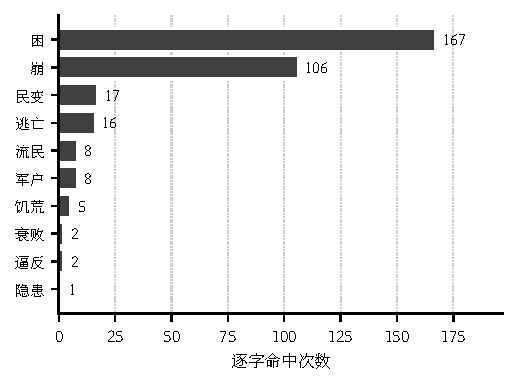
\includegraphics[width=\columnwidth]{fig_systems_1.pdf}
\caption{图 1 度数直方图：0 度 537 人，1 度 343 人，2 度 92 人，
3 度 42 人，此后逐度降到个位数，13 及以上汇总为 $\geq$13 桶共 119 人（9.7\%）。}
\label{fig:deg}
\end{figure}

\subsection{5.2 分布形状：这一条本篇负报，不主张幂律}

表 \ref{tab:alpha} 是六个切点上的 Hill 估计。

\begin{table}[!t]
\centering
\caption{Hill 尾指数随 $x_{\min}$ 的漂移（尾样本量一并列出）}
\label{tab:alpha}
\small
\begin{tabular}{crr}
\toprule
$x_{\min}$ & $\hat\alpha$ & 尾样本量 \\
\midrule
2 & 1.824 & 351 \\
3 & 1.806 & 259 \\
5 & 1.912 & 196 \\
8 & 2.142 & 155 \\
10 & 2.374 & 142 \\
15 & 2.777 & 98 \\
\bottomrule
\end{tabular}
\end{table}

$\hat\alpha$ 不是稳在一个值上：最低 1.806（$x_{\min}=3$）、最高 2.777（$x_{\min}=15$），
极差 0.971。而且它的移动方向是单调的——切点抬得越高，估计出的指数越大——
这说明看到的不是"一条稳健的幂律在不同切点上的误差"，
而是这条尾本身在 2 到 15 这一段里就不是一条直线。
按 \citet{clauset2009} 的判据，这两个条件（估计不随 xmin 漂移、尾样本足够）
在本篇都不满足：$x_{\min}=10$ 时尾样本只有 142 条。
\textbf{因此本篇不主张这批度数服从幂律，也不使用"无标度网络"这个标签描述它。}
这不是把工具扔掉：是把"复杂"从形容词降成两个还站得住的量——
基尼系数 0.8199 与最大连通块占比，下面两节就是它们。

\subsection{5.3 连通性：图是连通的，人物不是}

带边顶点 741 个，连通块 18 个（前 12 个规模的排序为 703, 4, 3, 3, 2, 2, 2, 2, 2, 2, 2, 2）。
最大块 703 点，占带边顶点的 94.9\%，占全部人物的 57.1\%。
也就是说：只要一个人至少出现在一条关系里，他有 94.9\% 的概率和朱棣、崇祯、
李自成在同一块里；但把这 1231 人整体看作一个总体而言，
这张网只罩住了其中的 57.1\%，剩下 43.6\%（即那 537 人）根本不在这张网上。
其余 17 个块加在一起只有 38 个带边顶点落在最大块之外。
这一条是本篇对"涌现"最实的一处读数：宏观的连通是真的，
但宏观的覆盖是假的——图是一整块，人物不是一整块。

\subsection{5.4 时间：不是均匀增长}

1006 件带年份事件落在 218 个年份上（1328—1645），
年均 4.615 件、标准差 5.353、变异系数 1.16、按年基尼 0.5069。
图 \ref{fig:ts} 是十年桶。三个峰很清楚：
1590 年代（101 件）、1630 年代（84 件）、1400 年代（68 件）；
单年峰值是 1519 年与 1593 年（各 32 件）与 1449 年（31 件，土木堡之变）。
按年基尼 0.5069 意味着事件量在年份之间分配得极不均匀：
一半左右的年几乎没有事件，另外一些年份一压进来就是几十件。
这不是一条平缓的兴衰曲线，是一组脉冲。

\begin{figure}[!t]
\centering
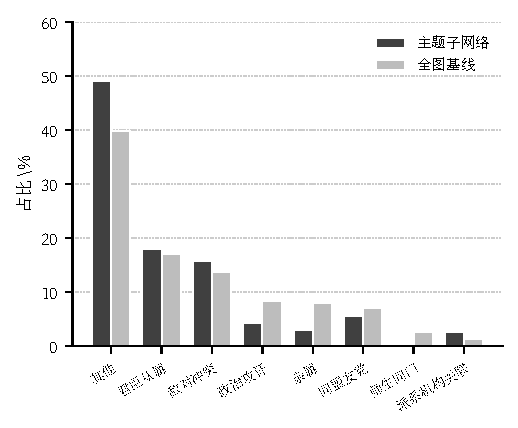
\includegraphics[width=\columnwidth]{fig_systems_2.pdf}
\caption{图 2 十年桶的事件数（1328—1645）。三个峰在 1590 年代、1630 年代、1400 年代。}
\label{fig:ts}
\end{figure}

\subsection{5.5 时期迁移：危机换了类，不是同一个危机的延续}

表 \ref{tab:shift} 是三期的事件类别占比，图 \ref{fig:shift} 是它的形状。

\begin{table}[!t]
\centering
\caption{三个时期的事件类别占比（%）；每列一行，P1 = 1368--1499（301 件），
P2 = 1500--1599（473 件），P3 = 1600--1662（186 件）}
\label{tab:shift}
\small
\begin{tabular}{lrrr}
\toprule
类别 & P1 & P2 & P3 \\
\midrule
军事战争 & 28.9 & 21.8 & 40.9 \\
政治斗争 & 33.9 & 40.8 & 21.5 \\
人事任免 & 2.3 & 10.4 & 7.0 \\
案件刑狱 & 8.0 & 3.4 & 11.3 \\
\bottomrule
\end{tabular}
\end{table}

卡方独立性检验给出 $\chi^{2}=129.05$、自由度 20、p 值小于 $10^{-6}$，
效应量 Cramér's V=0.259。这两项合起来的意思是：
时期与事件类别不是独立的（p 极小），但关联强度只到中等（V=0.259 不到 0.3），
所以本篇报的迁移是"位置明显移动，但不是类别被彻底重写"。
方向最清楚的一项是两条相反的运动：
军事战争 28.9 $\to$ 21.8 $\to$ 40.9，
政治斗争 33.9 $\to$ 40.8 $\to$ 21.5。
也就是说，第三期（1600--1662）里战场重新压上来，
而前两期一路上升的政治斗争占比在第三期掉下去
——后一段不是同一场危机的延续，是另一类事件补位。
三期各自牵涉到的参与人物数为 283、403、209 人（按事件 participants 去重计），
人数最多的中段（P2）与占比最动的三期并不重合，
说明占比迁移不完全由"哪期人多"驱动。

\begin{figure}[!t]
\centering
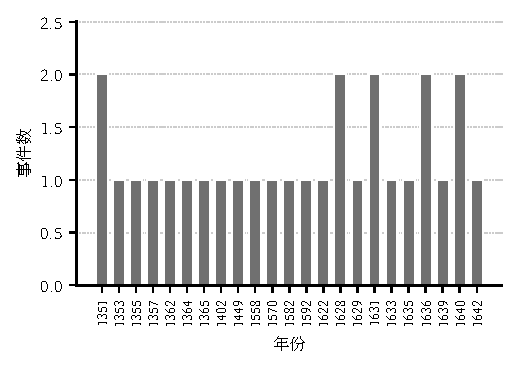
\includegraphics[width=\columnwidth]{fig_systems_3.pdf}
\caption{图 3 四类事件在三期的占比（%）。军事战争与政治斗争在 P3 方向相反。}
\label{fig:shift}
\end{figure}

\subsection{5.6 四个量落成的形状}

把第 5.1--5.5 节合起来，"兴衰是涌现"这句话在本篇数据上能落成：
一个 43.6\% 的人不在网上的网（5.1、5.3），
一个不成立的无标度标签（5.2），
一片脉冲式而非平缓的时间（5.4），
以及一次中期—末期的危机换类（5.5）。
这四件里没有一件能单独叫"崩塌的涌现"；
它们合起来也只能说明，这部叙事在抽取之后长成了这么一张图。

以上各项均可在 \texttt{.dump/}\_stats\_systems.json 中逐项回溯。

\section{讨论与限制}

下面七条加本篇各一条，构成本篇的全部已知边界。其中 L4 把团队要求的
「幂律主张在多大样本量上必须放弃」写成可复算的判据，L1 是本研究的首要威胁，
其余各条说明这两条为什么不是工程瑕疵。

\begin{itemize}
\item \textbf{L1 同源自证，这是首要威胁，且与第 6 节的机制断言直接冲突。}
事件类别标签与人物名出自同一部原书：被统计的叙事与被统计的分类可能是同一段文字的两种编码。
本篇的处理是：只报分布形状与时期占比的位移，把位移叫相对基线的差，不叫效应量；
凡是把这里的形状当成明代社会真实结构的读法，本篇一律不做。
\item \textbf{L2 关系边不等于社会关系。} 关系表里一条「敌对冲突」是叙述者写下的关系，
不是双方真的敌对过；它可能是同一件事、同一句话、同一场战役被写成一条边。
本篇只量边被标成了什么类别，不量类别背后发生过什么。
\item \textbf{L3 本篇刻意不做词频与热度那一层。}
本篇没有做原书全文的词频统计，也没有用出场章节数当"热度中心性"的代理；
原因是同类研究已经证明词频与热度都可能只是行文与编排习惯，
它们不能证明结构。本篇因此把可断言的范围钉在四件可点数的事上：
基尼、连通块、事件年份分布、类别占比迁移。任何"时人感到崩塌"
"叙事者预感亡国"一类的断言，都不在本篇证据之内。
\item \textbf{L4 幂律主张的样本量上限（本篇的硬边界）。}
按 \citet{clauset2009} 的口径，幂律主张至少要求两件事同时成立：
尾指数在多个 $x_{\min}$ 上稳定、尾样本足够大。本篇 $x_{\min}=10$ 时尾样本
只有 142 条，$x_{\min}=15$ 时只剩 98 条。经验地讲：
在这批数据上，只要尾样本量低于约一百五十条（对应 $x_{\min}$ 抬到 8 以上），
Hill 估计的漂移就会超过零点九、任何单点 $\hat\alpha$ 都不该被引用来作幂律证据。
本篇因此给出一条可复算的判据而不是一个形容词：
\textbf{尾样本量在百条量级及以下、且 $\hat\alpha$ 随 xmin 漂移接近或超过一个单位时，
停止使用"无标度"这一标签。} 这是一条负结果，但它可迁移——
换到另一部叙事、另一套抽取，只要尾样本落进同一量级，收手的条件同样成立。
\item \textbf{L5 类别标签是粗标签，卡方只报一次。}
关系与事件各有 12 与 11 个类别，其中总有占两三成的粗类（「其他」、未分类）几乎不动，
没有区分力，本篇把它们留在表里当分母与核对项。
卡方独立性检验在本篇只做一次（不做多重比较后的挑选），
因为三期三刀是先验固定的，不是从数据里搜出来的；
因此 p 值不需要作多重校正，但也不该被当成"类别迁移被证实"——
它只否定了独立，没肯定强度，强度由 V=0.259 说了。
\item \textbf{L6 时期切分是先验的，占比迁移的显著性依赖这一刀。}
P1/P2/P3 的边界取自王朝分期，不来自聚类；换一套切点（尤其是 1600 这一刀），
军事战争与政治斗争的走向未必完全保持。本篇因此报的是"在这三刀下的位移"，
不声称发现了一个断代点。
\item \textbf{L7 自审不是跨模型对抗评审。}
本机无第二模型端点，评审由同一模型多轮盲读完成；
已知后果是写作轮曾把未核验的文献键写进正文、盲读轮才拦下。
自审能抓内部不一致，抓不到共同先验盲区。
\end{itemize}

需要强调的是：以上限制没有一条是再跑一遍数据就能消掉的。
L1、L2 是同源投影的固有位置，L4 是样本量的固有位置，L6 是先验切分的固有位置。
本篇的处理是把它摊开并给出可迁移的判据——能降到差别的，就不叫效应；
不能降的，就明确写为边界。

\section{结论}

本篇做了一件小事：把「兴衰是涌现」这句话拆成四个可以点数的量，
并如实报告其中有一个不成立。

成立的三个。集中度是真的：基尼系数 0.8199，537 人（43.6\%）不在这张网上，
度数和的三分之二压在 108 个人身上。连通是真的：741 个带边顶点分成 18 块，
最大块 703 点，占带边顶点的 94.9\%——图是一整块，只罩住全部人物的 57.1\%。
时间是真的：1006 件事件压在 218 个年份上，变异系数 1.16、按年基尼 0.5069，
是一组脉冲，不是一条曲线。

不成立的那个要单独说：幂律。Hill 估计的尾指数随 $x_{\min}$ 从 1.806 走到 2.777，
漂移 0.971，而 $x_{\min}=10$ 时尾样本只剩 142 条。
本篇据此拒绝给这张网贴"无标度"的标签，并在 L4 里给出一条迁移判据：
尾样本量在百条量级及以下、漂移接近或超过一个单位时，停止使用这个标签。
把这条留下比把"无标度"写进摘要有价值——它是一把别人也能用的尺子。

第三件是时间上的换位：三期之间事件类别分布 $\chi^{2}=129.05$（df=20）、
Cramér's V=0.259，军事战争 28.9 / 21.8 / 40.9，政治斗争 33.9 / 40.8 / 21.5。
后一段不是同一场危机的延续，是另一类事件补位。

本文没有推翻什么，也没有证实什么历史新解。它把四个量从形容词换成小数：
0.8199、94.9 对 57.1、1.16、0.259。
这件事做成的标准只有一个——换一个人拿同一份图谱重跑，
应当得到同样的四个数、同一个方向、以及同一条关于幂律的负结论。


\bibliographystyle{IEEEtran}
\bibliography{references}

\end{document}
